\DiaryEntry{1000 Problems in Probability, 3}{2018-12-18}{Stochastic}

\subsection{Section 3.8, Problem 3}

We have two RVs $X, Y$ each with geometric distribution and parameter $\alpha$ and $\beta$, respectively. Calculate the pmf of the sum $Z = X+Y$. The pmfs are $f_X(k) = \alpha(1-\alpha)^k$ and $f_Y(k) = \beta(1-\beta)^k$. The pdf of their sum is given by

\bee
f_Z(z) = \sum_{k=0}^z \alpha (1-\alpha)^k \beta (1-\beta)^{z-k} = \alpha \beta (1-\beta)^z \sum_{k=0}^z \left( \frac{1-\alpha}{1-\beta}\right)^k
\eee

We can sum this by means of the geometric series equation and obtain (after some algebraic transformations)

\bee
f_Z(z) = \alpha \beta (1-\beta)^z \frac{1 - \left( \frac{1-\alpha}{1-\beta}\right)^{z+1}}{1 - \frac{1-\alpha}{1 - \beta}} = \cdots = \frac{\alpha \beta}{\alpha-\beta} \left[ (1-\beta)^{z+1} - (1-\alpha)^{z+1}\right]
\eee

The following plot shows the pmf $f_Z$ for $\alpha=0.2, \beta=0.3$. The pmf starts at $0.06$, increases to some value around $k=3$ and then falls off: The geometric RV has a high probability for small values, therefore very small values ($< 3$) for the sum are unlikely. Conversely, the peak around $k=3$ is precisely caused by the preference for small values of the geometric RVs.


\begin{figure}[H]
  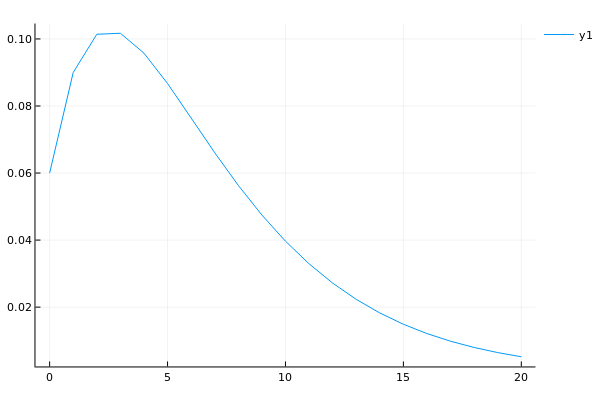
\includegraphics[scale=0.6]{images/1000_problems_in_prob_3_1.png}
\end{figure}




%%% Local Variables:
%%% mode: latex
%%% TeX-master: "journal"
%%% End:
